\documentclass[a4paper]{article}

\usepackage{graphicx,url,fullpage,fourier}
\textwidth=18.5cm
\oddsidemargin=-1.2cm
\textheight=26cm
\topmargin=-1.52cm
\usepackage{listings,color,hyperref,picinpar}

\lstset{language=C}
\definecolor{gris}{rgb}{0.95,0.95,0.95}
\definecolor{mygreen}{rgb}{0,0.6,0}
\definecolor{mygray}{rgb}{0.5,0.5,0.5}
\definecolor{mymauve}{rgb}{0.58,0,0.82}

\lstset{ %
  backgroundcolor=\color{gris},
  basicstyle=\footnotesize,   
  breakatwhitespace=false,   
  breaklines=true,          
  captionpos=b,            
  commentstyle=\color{mygreen},
  deletekeywords={...},       
  escapeinside={\%*}{*)},          % if you want to add LaTeX within your code
  extendedchars=true,        
  frame=single,             
  keepspaces=true,         
  keywordstyle=\color{blue},
  language=Octave,       
  morekeywords={*,...}, 
  numbers=left,        
  numbersep=5pt,      
  numberstyle=\footnotesize\color{mygray}, 
  showspaces=false,   
  showstringspaces=false,
  showtabs=false,       
  stepnumber=2,         
  stringstyle=\color{mymauve},
  tabsize=2,                 
  title=\lstname                   % show the filename of files included with \lstinputlisting; also try caption instead of title
}

\begin{document}
\begin{center}
{\bf \Large Quartz tuning fork resonator stroboscopic displacement field mapping}\\ \ \\
J.-M Friedt, \today
\end{center}

Quartz resonators are core components in all systems requiring a clock signal -- most significantly
all synchronous digital systems (i.e. microprocessors/microcontrollers). While bulk acoustic resonators
are available for frequencies ranging from a few hundred kHz to a few hundred MHz (using overtones),
the most common quartz resonator geometry is the tuning fork. This geometry, used in all so called
quartz watches \cite{slom}, has evolved from the basic beam geometry to eliminate unwanted modes by using 
symmetry considerations to cancel symmetric modes. Odd overtones are well separated in frequency to be electrically filtered.
Hence, a mechanical vibration is the basic underlying principle of most stable watches, with the drawback 
of a sensitivity to environmental conditions changing the acoustic velocity of the quartz substrate -- most
significantly temperature -- yielding to some long term drift compensation strategy as found in atomic clocks.
The topic we wish to address in this laboratory session is mapping the displacement of the quartz tuning fork
resonator, along the beam length and depending on the frequency.

\noindent
\fbox{\parbox{\linewidth}{This laboratory experiment only requires a computer fitted with a sound card sampling at 192~kHz, a USB bus,
a webcam, and less than 10~euro worth of electronic components. It is designed to be easy to reproduce.}}

\section{Introduction}

While a resonator is classically used in a closed loop configuration as an oscillator, characterizing
the spectral characteristics of the tuning for is most easily achieved by using an open-loop approach
\cite{jm0,jm1}. Commercial
instruments -- network analyzers -- perform this task extremely well, but are expensive and do not provide the
signals needed to visually observe the displacement of the prongs. Hence, our first objective is to assemble a 
stable signal source: the source must exhibit a better frequency stability than the object under investigation.
Considering the excellent frequency stability of quartz resonators and their high quality factor, only a quartz
controlled synthesizer (as opposed to a LC low-frequency generator) provides the targeted stability. One such generator is a sound
card \cite{jm2}. Furthermore, stereo sound cards are ideally suited to the targeted purpose: one channel will be used to power
the tuning fork and the second channel will drive the voltage of a LED used to illuminate the tuning fork prongs in order
to achieve a stroboscopic lighting. Hence, any low-cost webcam with an exposure duration longer than the oscillation
period will allow visualizing the prong motion, at an equivalent frequency equal to the difference of the frequencies
between the signals driving the tuning fork and driving the light source \cite{jm3}.

The MEMS characterization tool we will develop during this laboratory session is a simplified
version of such fancy instruments as Poytec's MSA-500 Micro System Analyzer as shown at
\url{http://photonic-technologies.info/eu/products/vibration-sensors/microscope-based-systems/msa-500-micro-system-analyzer/}.

\begin{figwindow}[1,r,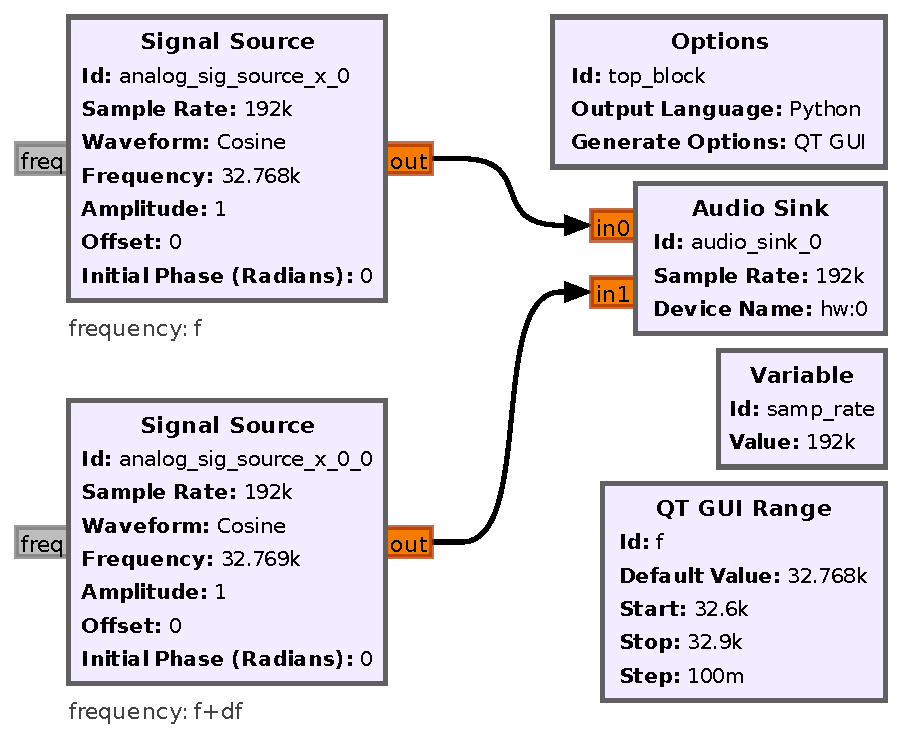
\includegraphics[width=0.39\linewidth]{audio.pdf}, %audio_grc.png},
{GNU Radio flowchart for programming the two stereo outputs with a given user-defined frequency, one of the
channels being offset by 1-Hz with respect to the other.}\label{grc}]
The opensource GNURadio framework allows for defining both stereo channel frequencies, sweeping the frequency source,
and keeping a constant offset between both channel frequencies (Fig. \ref{grc}). However, the stroboscopic illumination pulse must
be short with respect to the period. While a 192~kHz sampling rate meets Nyquist criterion when generating a $32768=2^{15}$~Hz
signal -- the nominal resonance frequency of most tuning forks -- it will not be sufficient to generate a pulse lasting
about 1/10th of the period. Hence, a dedicated pulse generation circuit must be assembled to drive the LED.
\end{figwindow}

{\bf
\begin{enumerate}
\item A tuning fork resonance frequency is 32768~Hz. Find a quartz tuning\\
fork datasheet: what is the typical quality factor of a packaged tuning \\
fork~? what is the frequency resolution needed to observe the\\ resonance 
in a network analyzer configuration~?
\item When the tuning fork package is opened and the vibrating element \\
exposed to air, the quality factor drops 10-fold due to viscous drag. \\What 
is the frequency resolution needed to observe the resonance \\
frequency once  the sealed packaging has
been opened~?
\item What is a stroboscopic illumination strategy to observe objects moving quickly but periodically~?
\end{enumerate}
}

\section{Stroboscopic signal generation}

A stroboscopic signal meets two requirements:
\begin{itemize}
\item the period is close to the driving signal: the frequency difference between the device-under-test
driving signal and the stroboscopic signal defines the speed at which the phenomenon under investigation is observed.
\item the duration of the illumination is ``much'' shorter than the period to give the feeling that each 
frame is frozen in time. Too long an illumination with respect to the phenomenon period will blur the image.
\end{itemize}

\begin{figwindow}[0,r,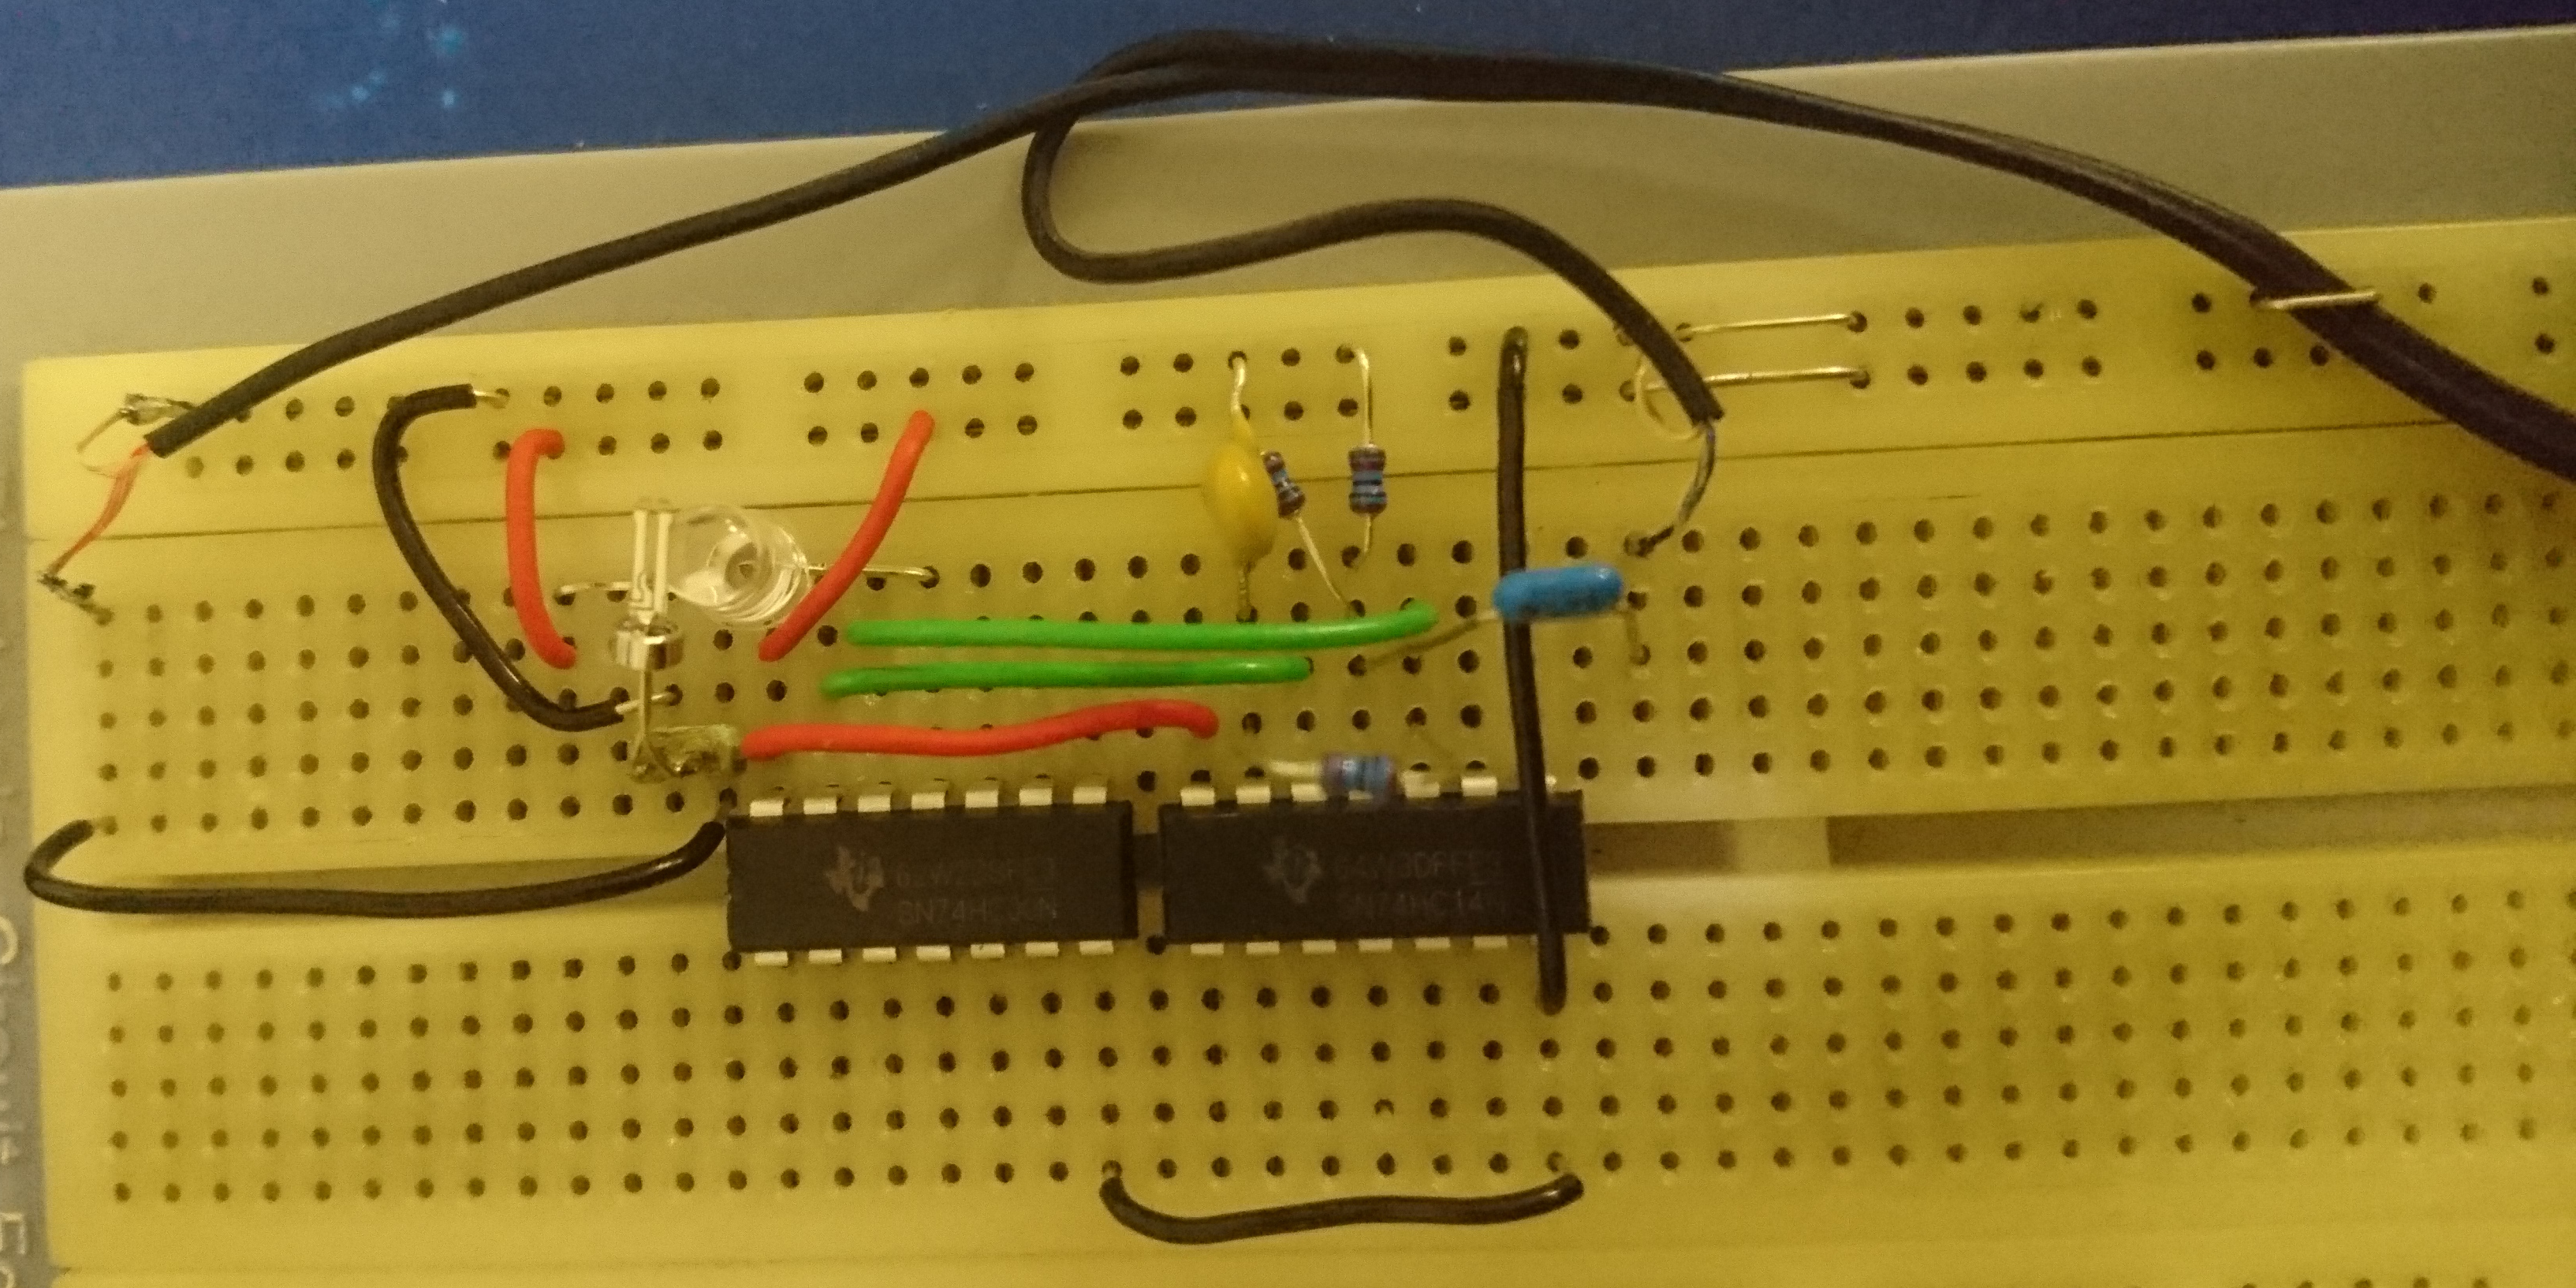
\includegraphics[width=0.4\linewidth]{DSC_2946.JPG},{Assembled stroboscopic signal
generation circuit}\label{2}]
Generating the pulse driving the LED must be addressed at the hardware level (Fig. \ref{2}). 
One classical method for generating short pulses
is to use two Schmitt triggers: the sine wave generated by the sound card is converted to a square
wave using the first stage of a Schmitt trigger. This square-shaped signal feeds an RC circuit with a time 
constant tuned so that it is small with respect to the incoming signal period. The output of the RC circuit 
feeds a Schmitt trigger which converts the exponentially decaying signal to a square wave, delayed by the 
time needed to reach the threshold voltage. Having two square waves, one resulting from the original sine-wave 
and the second with a RC-delayed copy of this signal, we generate the pulses driving the LED as an AND 
function between both pulses.
\end{figwindow}

{\bf
\begin{enumerate}
\setcounter{enumi}{3}
\item Considering the period of the signal driving the tuning fork, what is the RC time constant needed 
for the stroboscopic signal~?
\item the sound card signal is centered on 0~V (AC signal) while the Schmitt trigger requires a signal 
below a few 100~mV to remain to 0 and otherwise raises its output to the supply voltage. The AC-coupled 
sound card output is DC-offset using a resistor bridge. To prevent DC-leakage to the sound card output 
amplifier, a capacitor is introduced. What is the impedance of a capacitor as a function of frequency~? 
select the appropriate capacitor value as a function of the polarizing resistor bridge. What are the 
conditions for a voltage divider resistor bridge to operate properly~?
\item Select appropriate component references to assemble the circuit: what integrated circuits provide
the necessary functions~?
\end{enumerate}
}

Two chips are provided in DIL packages: the 7414 Schmitt trigger and the 7400 AND gate. 

{\bf
\begin{enumerate}
\setcounter{enumi}{6}
\item After reading the datasheet of these chips, what is a wiring schematic suitable for implementing the
pulse generator driving the LED~?
\item Simulate the circuit using {\tt ngspice}. The inverting NAND gate can be simulated using the {\tt hyst} function:
\begin{verbatim}
.model schmitt hyst(in_low=1.49 in_high=3.51 hyst=0 out_lower_limit=5.0 out_upper_limit=0.0 
+ input_domain=0.01 fraction=TRUE)
\end{verbatim}
called in the circuit model with
\begin{verbatim}
a1 1 2 schmitt
\end{verbatim}
\end{enumerate}
}
The result of the SPICE simulation should look like Fig. \ref{spice}.

\begin{figure}[h!tb]
\begin{center}
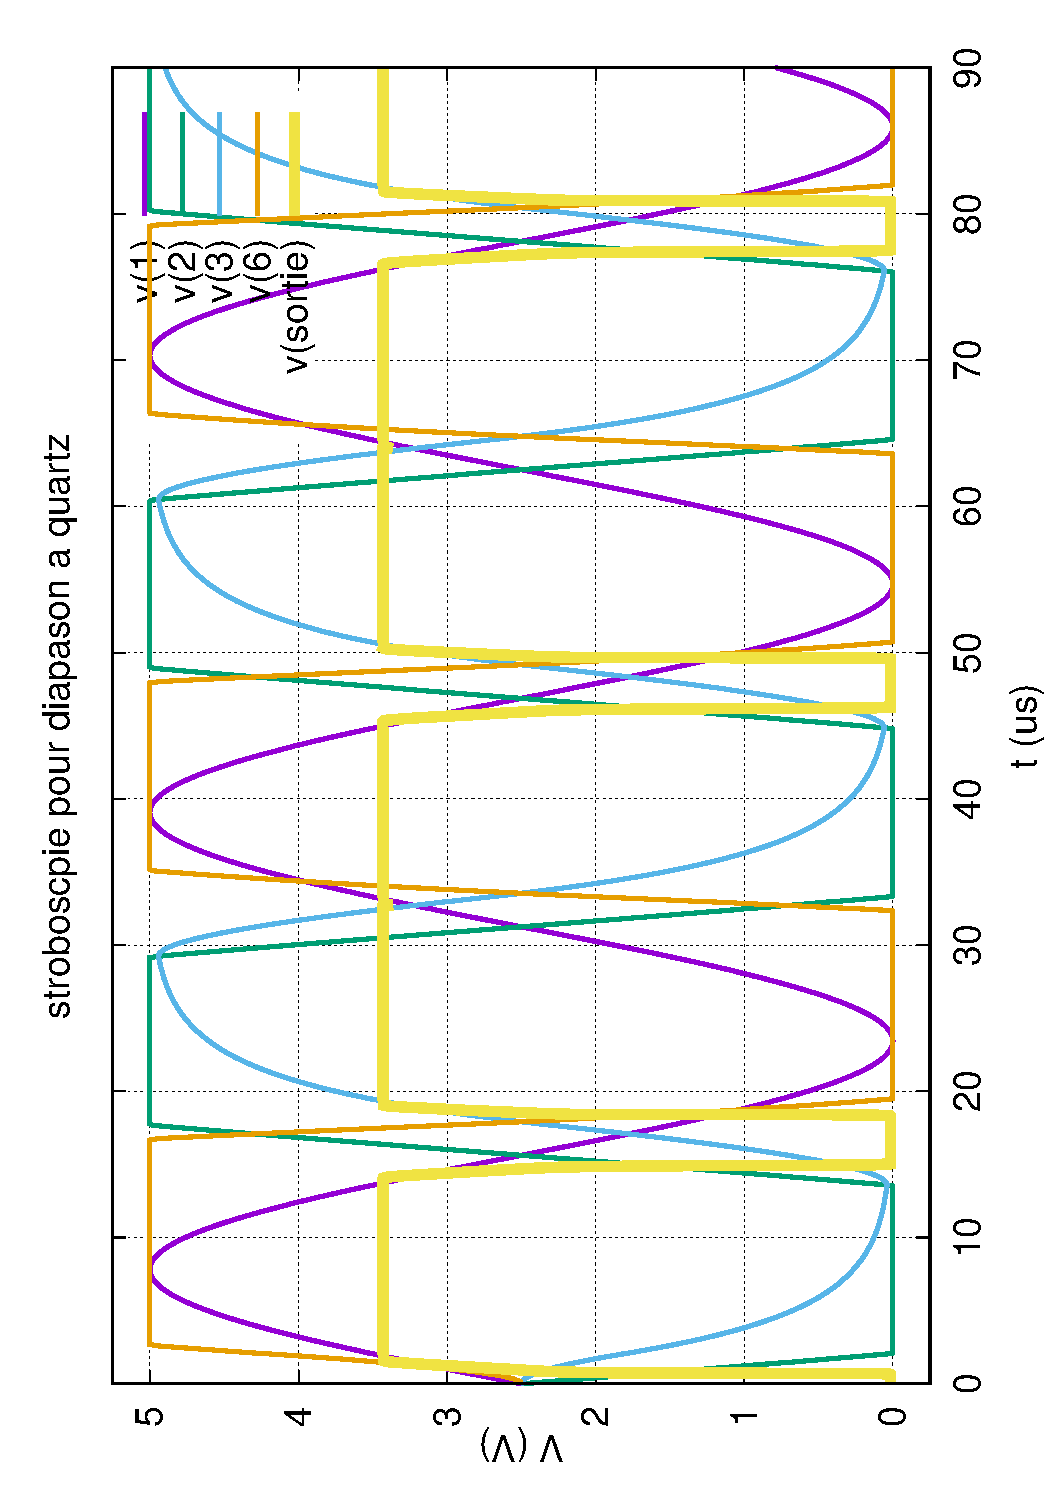
\includegraphics[angle=-90,width=0.62\linewidth]{simu_spice_sortie.pdf}
\end{center}
\caption{Simulation of the stroboscopic generation circuit using {\tt ngspice}. The bold line is the signal at the
output of the pulse shaping circuit driving the LED under control of the purple input sine wave.}
\label{spice}
\end{figure}

\section{Observing the prong motion}

Once the electronic boards have been setup on a breadboard, the tuning fork is located between the LED
and the webcam used to collect pictures of the tuning fork.

\noindent\fbox{\parbox{\linewidth}{The tuning fork prongs are extremely fragile: they are made of
300~$\mu$m thick quartz~! handle with care, and make sure the prongs never hit a wire or the LED when inserting
on the breadboard.}}

\begin{figure}[h!tb]
\begin{center}
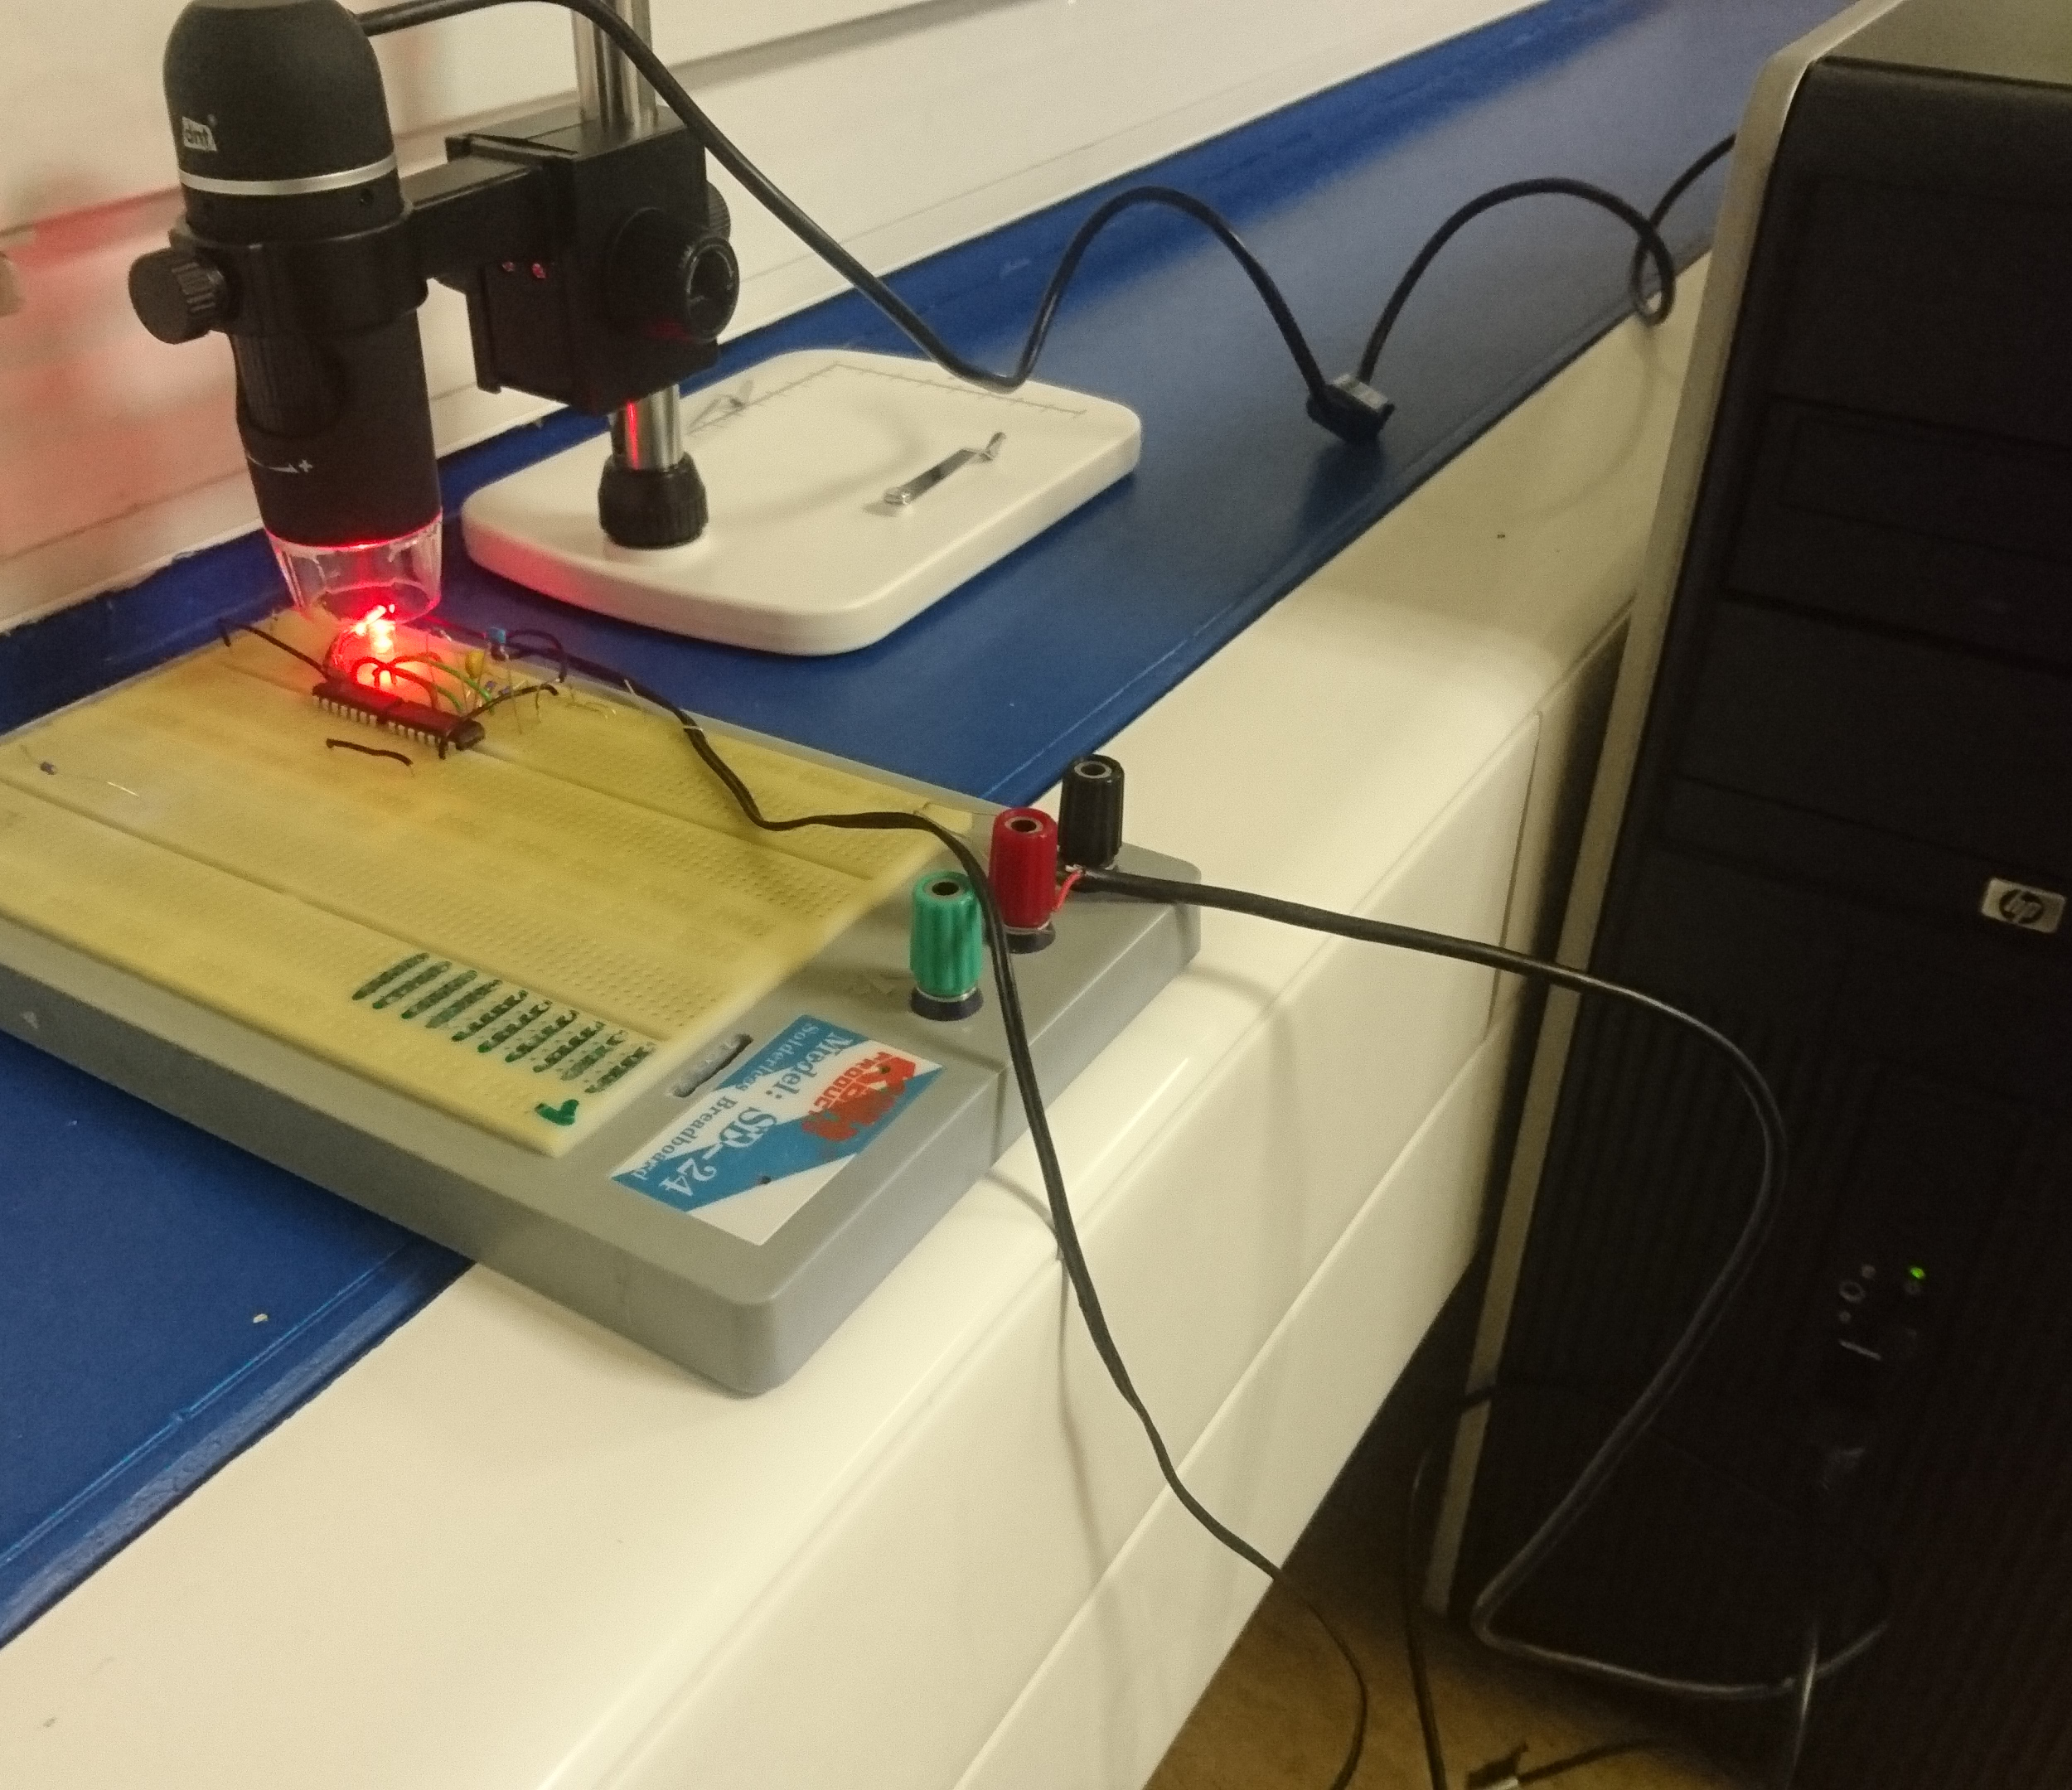
\includegraphics[height=4.4cm]{DSC_2942.JPG}
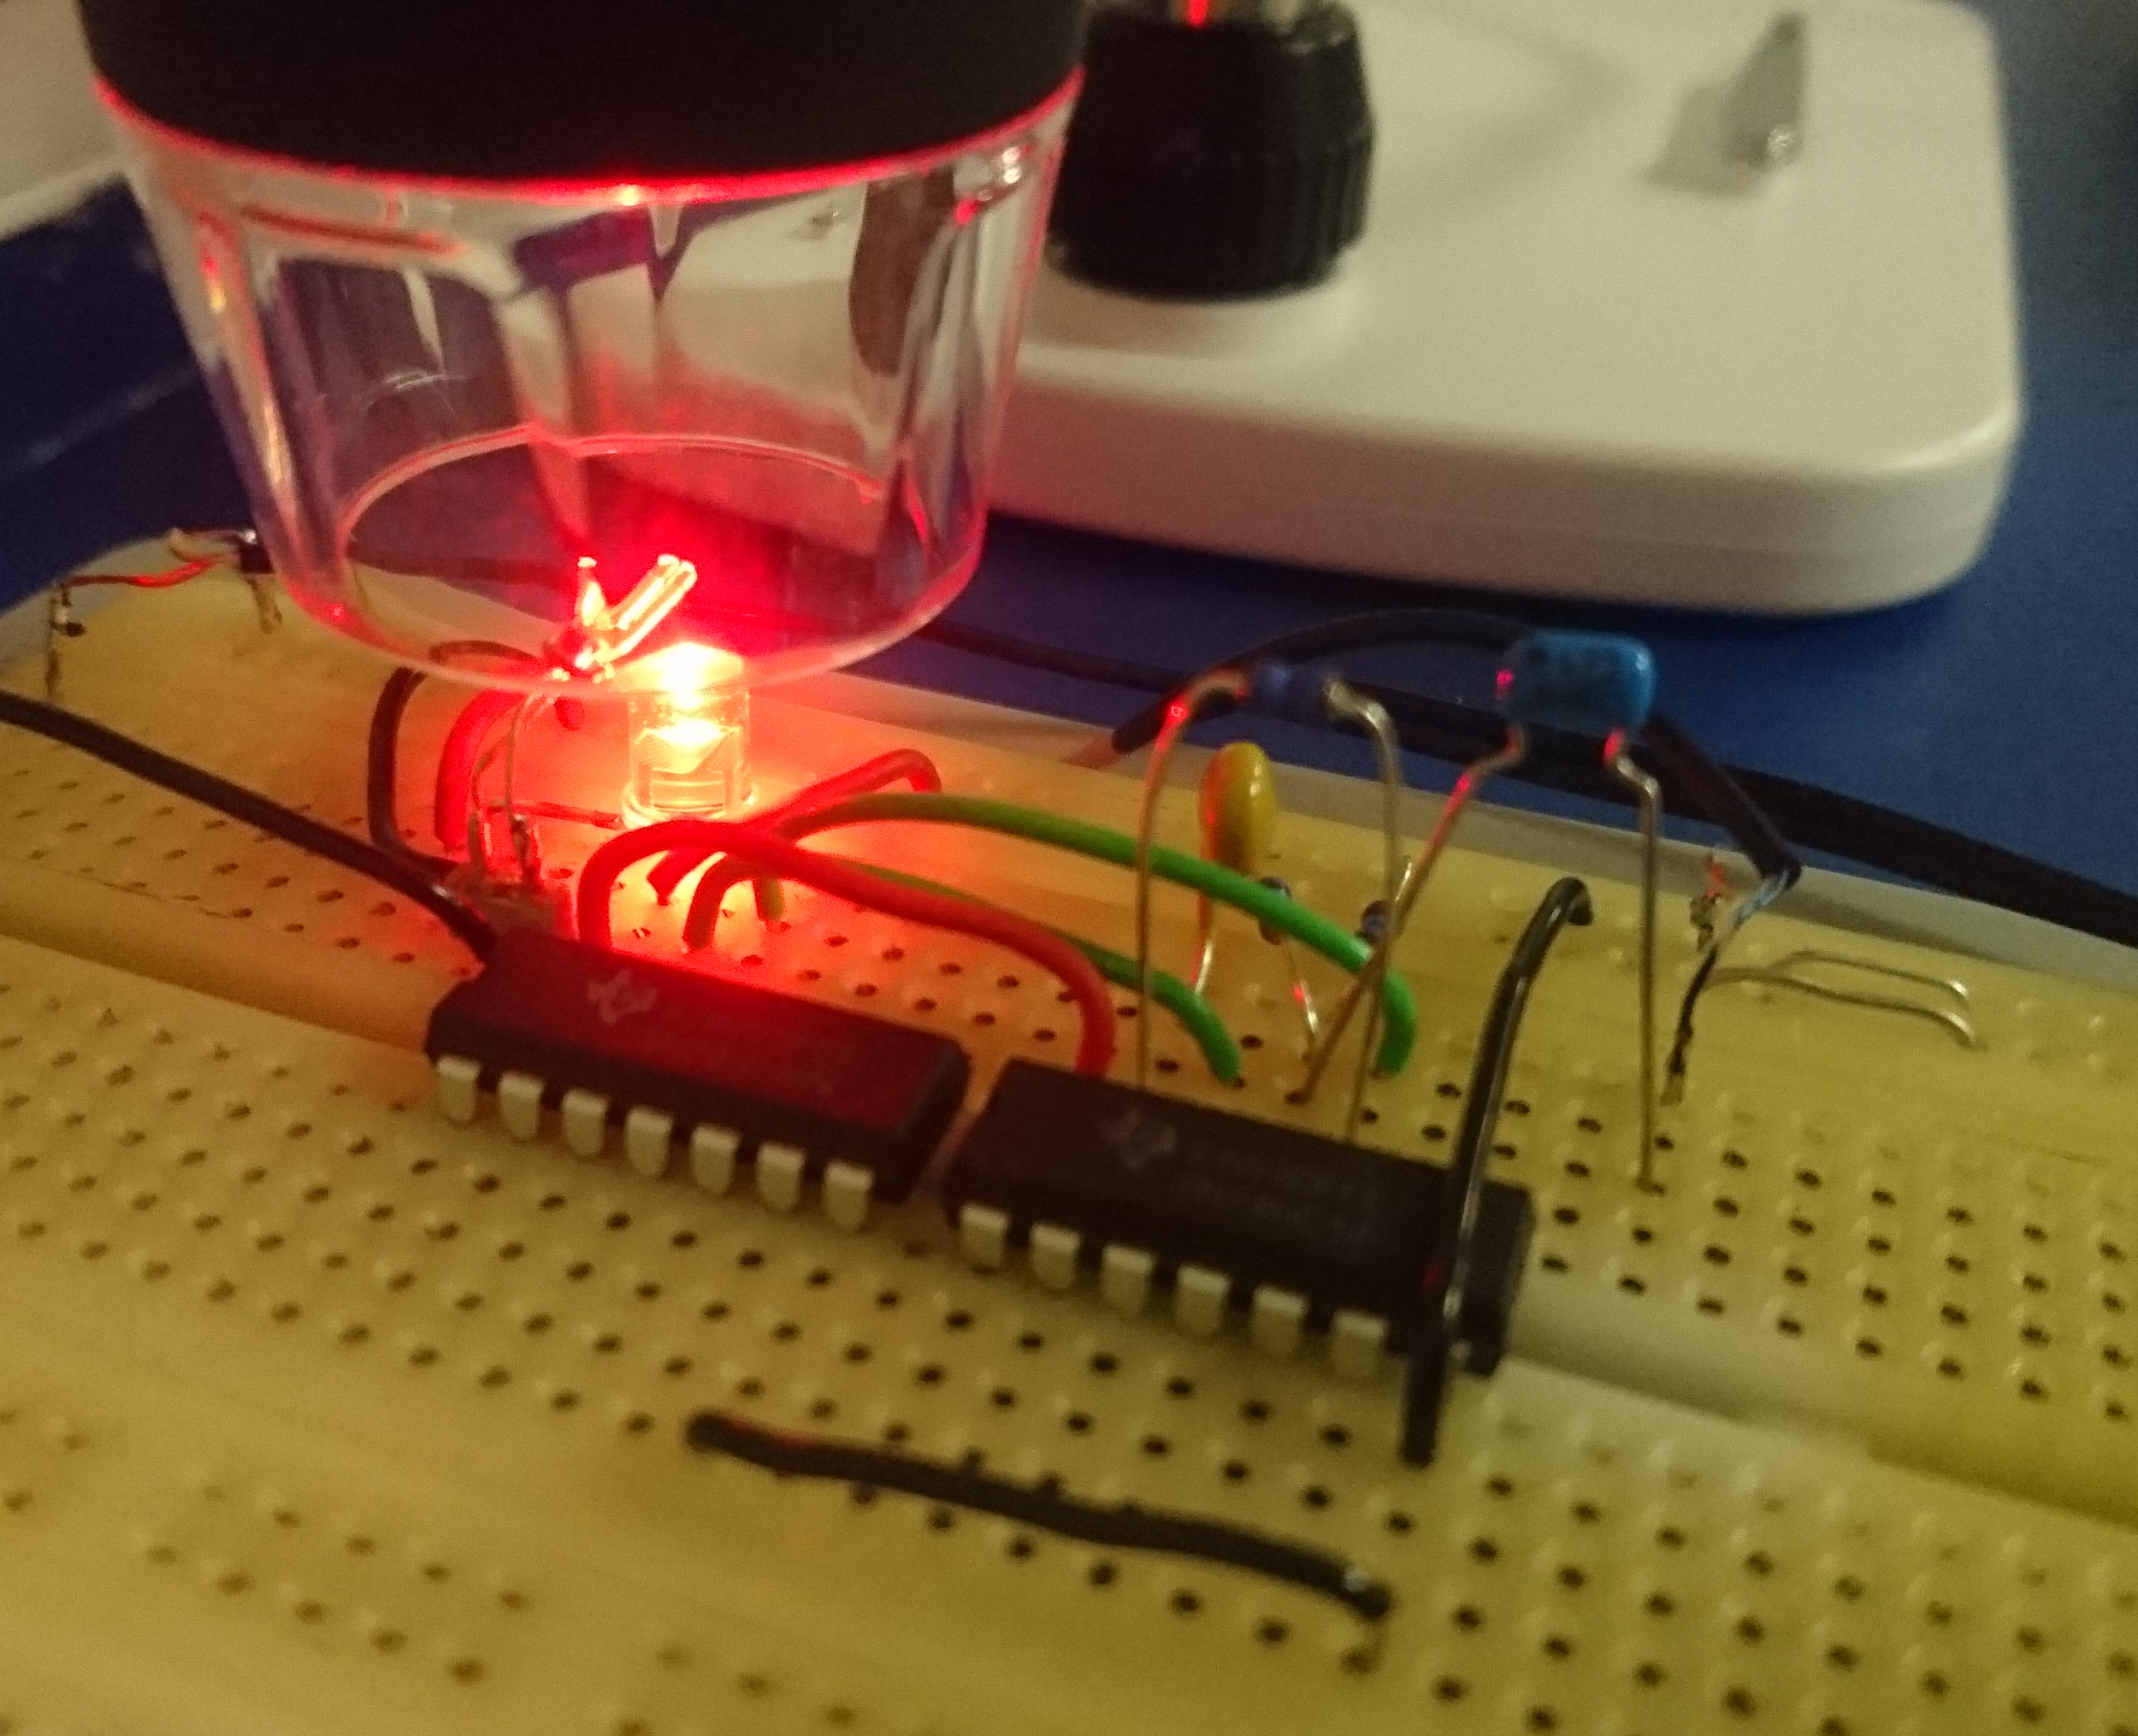
\includegraphics[height=4.4cm]{DSC_2943.JPG}
\end{center}
\caption{Experimental setup for observing the tuning fork prong oscillation: one sound card output 
drives the tuning fork, while the other output offset by 1~Hz drives the LED stroboscopic signal.}
\label{3}
\end{figure}

\noindent\fbox{\parbox{\linewidth}{In case the sound card is unable to generate 32760~Hz, either because
sampling at 48~kHz or because of a low pass filter when sampling at higher frequency, or if a stronger
driving amplitude is desirable, we might insert a Schmitt trigger before the tuning fork and drive with
a 5-V square wave rather than the direct sound card output. The stronger signal can also drive the tuning
fork using the third harmonic, hence setting GNU Radio audio out frequency to one-third of the tuning fork
resonance frequency. Achieving such a result requires duplicating the bias T circuit on another Schmitt trigger
of the same chip:

\begin{center}
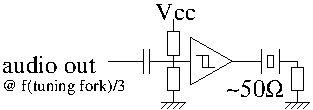
\includegraphics[width=.3\linewidth]{troisieme}
\end{center}
}}
\vspace{0.2cm}

Collecting the movie from the webcam is most easily achieved using VLC or {\tt xawtv} -- the former seems to sometimes exhibit excessively slow framerates and the latter seems
better suited to high-resolution webcams. 

Using the former software, the menu {\tt Media} $\rightarrow$ {\tt Open Capture Device} 
allows for selecting the {\tt Video Device Name}. Select {\tt /dev/video0}. After a few 
seconds, the webcam output should be visible on VLC. Switch off the white LED surrounding 
the lens if needed, and adjust the focus of the lens on the tuning fork. Once the tuning 
fork is well visible, sweep the frequency until the motion of the tuning fork is observed 
on the movie.

When using {\tt xawtv} to view the output of the camera, recording the image stream
is achieved using a different software, namely {\tt ffmpeg}: kill {\tt xawtv} and
record the movie of the vibrating tuning fork with {\tt ffmpeg -f video4linux2 -i /dev/video0 movie.avi}. Alternatively to {\tt xawtv}, FFMPEG also provides a viewer as {\tt
ffplay -i /dev/video0}.

{\bf
\begin{enumerate}
\setcounter{enumi}{7}
\item Considering the tuning fork quality factor, we have already addressed the frequency step needed to
observe the resonance. How quickly can the frequency vary, considering the settling time of the vibration, when
searching for the resonance frequency by sweeping the sound card output frequency~?
\end{enumerate}
}

The set of software needed to run the experiment is shown in Fig. \ref{scrt}: sound level is tuned using
{\tt alsamixer}, sound generation at 192~kS/s is driven by GNURadio and its graphical user interface
{\tt gnuradio-companion}, and image capture is achieved using VLC or ffplay. Once the oscillation is observed, 
a movie is recorded using {\tt Playback} $\rightarrow$ {\tt Record} or ffmpeg. We only need a few seconds worth
of movie, so quickly stop the record to keep the file size reasonable.

\begin{figure}
\begin{center}
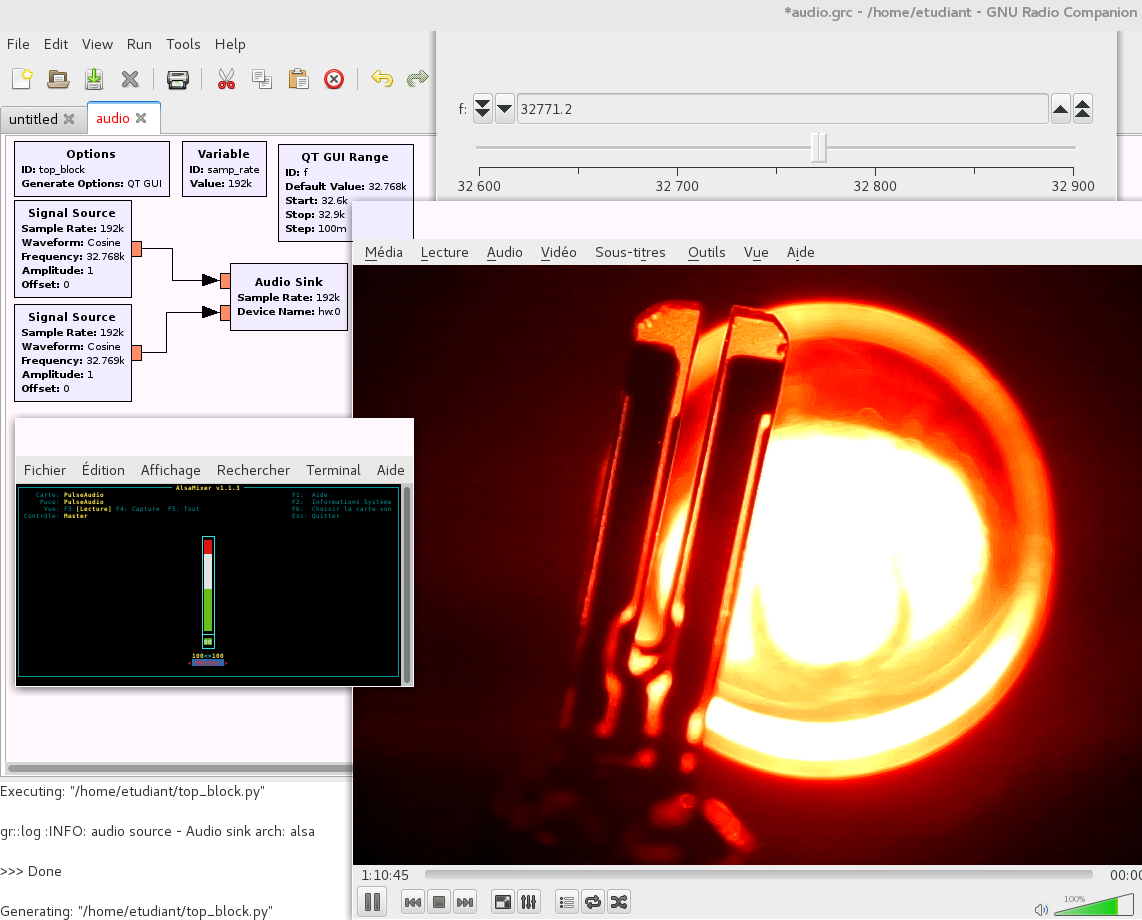
\includegraphics[width=0.51\linewidth]{tp_diapason.png}
\end{center}
\vspace{-0.4cm}
\caption{All the tools needed to drive the circuit and acquire the data: top-left is 
the GNURadio flowchart defining the soundcard output signals, top-right is the slider for defining 
the driving signal frequency, bottom-right is the video acquisition software displaying the webcam output
(VLC) and bottom-left is the driving voltage level tuner -- {\tt alsamixer}. The movie version of this
screenshot is at \url{jmfriedt.free.fr/recordmydesktop_tp_tuningfork.ogv}.}
\label{scrt}
\end{figure}

\section{Image processing}

\begin{figwindow}[0,r,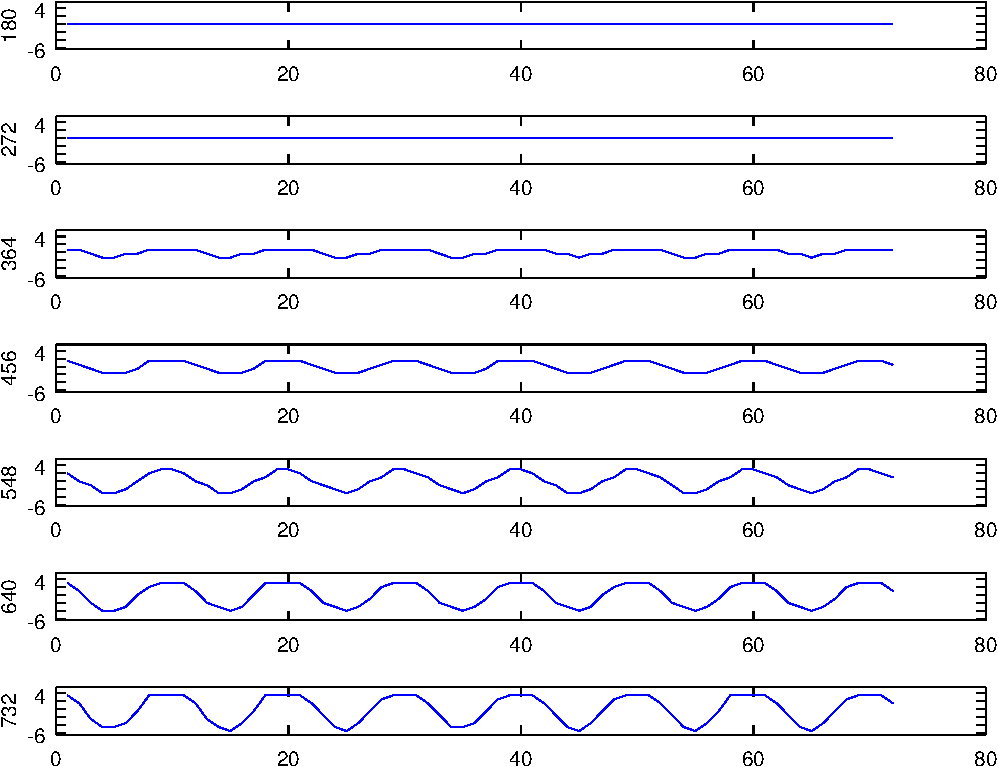
\includegraphics[width=0.49\linewidth]{fig6b},{Tuning fork displacement, in pixel, along the prong length. The prong is clamped at its
upper position which does not move, and the fundamental mode exhibits maximum vibration at the opposite
end of the prong.}\label{fig6}]
Quantitative analysis of the prong motion is addressed using digital image processing. The movie
is converted to a set of individual pictures using for example {\tt mplayer -vo jpeg movie.avi}. Alternatively,
{\tt ffmpeg} can also complete the task, as discussed in the man page. A suitable framework for
image processing is GNU/Octave with its Image Processing toolbox: a color image is read with
{\tt x=imread('imagename.jpg');} 
and converted to a greyscale image by keeping
only the red component: {\tt x=x(:,:,1);}. The prong can be rotated parallel to one of the image axis
by using {\tt imrotate()}.
\end{figwindow}\vspace{0.1cm}

{\bf
\begin{enumerate}
\setcounter{enumi}{8}
\item Motion is detected by searching for matching patterns in \\a ``small'' region of interest between successive images. \\
What signal processing function is used to detect \\similar patterns between two signals~?
\item Apply this mathematical function to one line or \\
column of the picture displaying the end of the prong: \\
display the curve of the prong motion over time. The \\
result should look like on of the curves of 
Fig. \ref{fig6}.
\item Repeat the measurement for various frequencies around the resonance, and display the motion
amplitude as a function of frequency.
\end{enumerate}
}
%\vspace{-0.7cm}

\begin{thebibliography}{9}
\bibitem{slom} T. Hunkin \& R. Garrod, {\em Secret Life Of Machines:
The Quartz Watch} (1991), at \url{https://www.youtube.com/watch?v=nQ9_bOIj49s}
\bibitem{jm0} J.-M Friedt, \'E. Carry, {\em Introduction au diapason \`a quartz}, Bull. de l'Union des Physiciens {\bf 879} 1137--1146 (2005) [in French]
\bibitem{jm1} J.-M Friedt, \'E. Carry, {\em Introduction to the quartz tuning fork}, American Journal of 
Physics, pp.415-422 (2007)
\bibitem{jm2} J.Marc, C. Canard, A. Vailly, V. Pichery, J.-M. Friedt, {\em Le diapason \`a quartz comme 
capteur~: utilisation de la carte son de PC pour l'instrumentation}, Bull. de l'Union des Physiciens {\bf 958}, pp.1051--1073 (2013) [in French]
\bibitem{jm3} J.-M. Friedt, {\em Mesure stroboscopique du champ de d\'eplacement d'un diapason \`a quartz 
au moyen d'une carte son et d'une webcam}, Bull. de l'Union des Physiciens {\bf 999} (2017) [in French]
\end{thebibliography}
\end{document}
